\section{Risultati e Valutazione}
\label{cap4}
%\textit{The Results section is dedicated to presenting the actual results (i.e. measured and calculated quantities), not to discussing their meaning or interpretation. The results should be summarized using appropriate Tables and Figures (graphs or schematics). Every Figure and Table should have a legend that describes concisely what is contained or shown. Figure legends go below the figure, table legends above the table. Throughout the report, but especially in this section, pay attention to reporting numbers with an appropriate number of significant figures. }

In Figura \ref{fig:primiModelli} e Figura \ref{fig:secondiModelli} vengono riportati i risultati ottenuti sul train e validation set per \textit{loss} e \textit{accuracy} con i modelli precedentemente descritti.
Si può notare come, nonostante vari tentativi con diverse tecniche di regolarizzazione, nessuna rete abbia condotto a risultati soddisfacenti sul validation set.
Il principale problema riscontrato è la tendenza della \textit{validation loss} a una leggera crescita (ciò è osservarvabile in quasi tutti i modelli, nonostante le tecniche di regolarizzazione).
\begin{figure}[h!]
     \centering
     \begin{subfigure}[b]{0.32\textwidth}
         \centering
         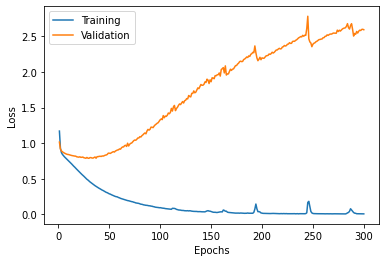
\includegraphics[width=\textwidth]{Latex template for Project Report-20220108/immagini/FAMDLoss.PNG}
         \caption{FAMD Loss}
         \label{fig:FAMDLoss}
     \end{subfigure}
     \hfill
     \begin{subfigure}[b]{0.32\textwidth}
         \centering
         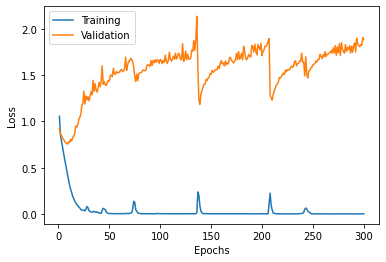
\includegraphics[width=\textwidth]{Latex template for Project Report-20220108/immagini/OHELoss.png}
         \caption{OHE Loss}
         \label{fig:OHELoss}
     \end{subfigure}
     \hfill
     \begin{subfigure}[b]{0.32\textwidth}
         \centering
         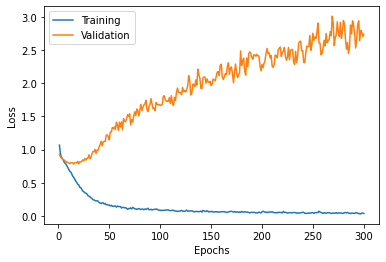
\includegraphics[width=\textwidth]{Latex template for Project Report-20220108/immagini/DropoutLoss.png}
         \caption{Dropout Loss}
         \label{fig:DropLoss}
     \end{subfigure}
     
     \begin{subfigure}[b]{0.32\textwidth}
         \centering
         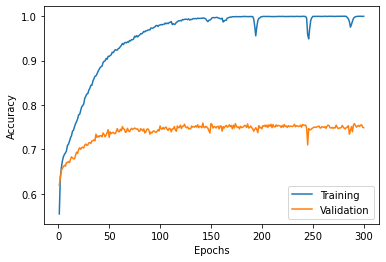
\includegraphics[width=\textwidth]{Latex template for Project Report-20220108/immagini/FAMDAccuracy.png}
         \caption{FAMD Accuracy}
         \label{fig:FAMDAcc}
     \end{subfigure}
     \hfill
     \begin{subfigure}[b]{0.32\textwidth}
         \centering
         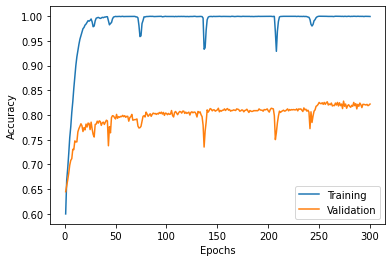
\includegraphics[width=\textwidth]{Latex template for Project Report-20220108/immagini/OHEAccuracy.png}
         \caption{OHE Accuracy}
         \label{fig:OHEAcc}
     \end{subfigure}
     \hfill
     \begin{subfigure}[b]{0.32\textwidth}
         \centering
         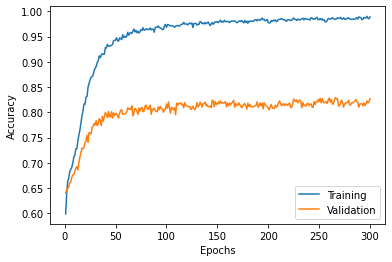
\includegraphics[width=\textwidth]{Latex template for Project Report-20220108/immagini/DropoutAccuracy.png}
         \caption{Dropout Accuracy}
         \label{fig:DropAcc}
     \end{subfigure}
     
     \begin{subfigure}[b]{0.32\textwidth}
         \centering
         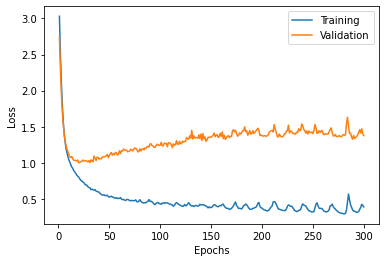
\includegraphics[width=\textwidth]{Latex template for Project Report-20220108/immagini/L1Loss.png}
         \caption{L1 Loss}
         \label{fig:L1Loss}
     \end{subfigure}
     \hfill
     \begin{subfigure}[b]{0.32\textwidth}
         \centering
         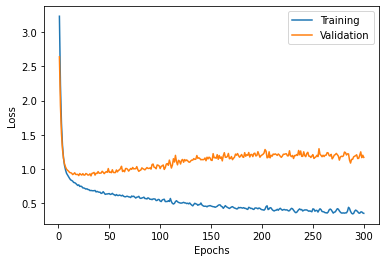
\includegraphics[width=\textwidth]{Latex template for Project Report-20220108/immagini/L2Loss.png}
         \caption{L2 Loss}
         \label{fig:L2Loss}
     \end{subfigure}
     \hfill
     \begin{subfigure}[b]{0.32\textwidth}
         \centering
         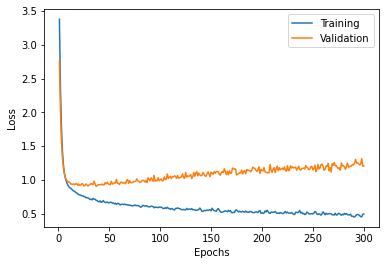
\includegraphics[width=\textwidth]{Latex template for Project Report-20220108/immagini/L2DropoutLoss.png}
         \caption{L2-Drop Loss}
         \label{fig:L2DropLoss}
     \end{subfigure}
     
     \begin{subfigure}[b]{0.32\textwidth}
         \centering
         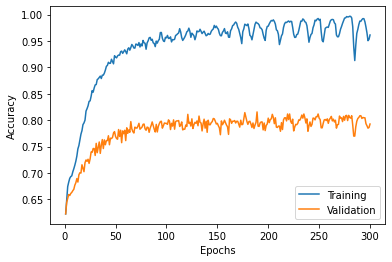
\includegraphics[width=\textwidth]{Latex template for Project Report-20220108/immagini/L1Accuracy.png}
         \caption{L1 Accuracy}
         \label{fig:L1Acc}
     \end{subfigure}
     \hfill
     \begin{subfigure}[b]{0.32\textwidth}
         \centering
         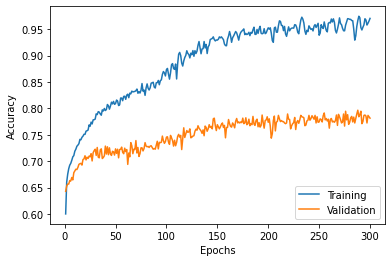
\includegraphics[width=\textwidth]{Latex template for Project Report-20220108/immagini/L2Accuracy.png}
         \caption{L2 Accuracy}
         \label{fig:L2Acc}
     \end{subfigure}
     \hfill
     \begin{subfigure}[b]{0.32\textwidth}
         \centering
         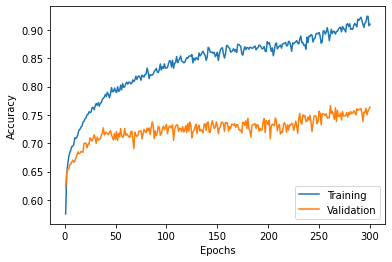
\includegraphics[width=\textwidth]{Latex template for Project Report-20220108/immagini/L2DropoutAccuracy.png}
         \caption{L2-Drop Accuracy}
         \label{fig:L2DropAcc}
     \end{subfigure}

     \caption{Loss e accuracy dei modelli ottenuti con e senza regolarizzazione}
     \label{fig:primiModelli}
\end{figure}
D'altro canto si può invece notare come l'andamento della \textit{validation accuracy} tenda correttamente a crescere (anche se in molti casi non in maniera decisa). Buoni risultati sono invece stati ottenuti sul training set sia per \textit{loss} che per \textit{accuracy}. Al fine di rendere più chiaro il risultato ottenuto all'ultima epoca da ogni modello, sono stati riportati nella Tabella \ref{tab:xxx} i valori di \textit{loss} e \textit{accuracy} per train e validation set.

\begin{figure}[h!]
     \centering
    \begin{subfigure}[b]{0.32\textwidth}
         \centering
         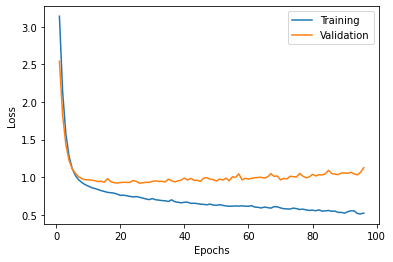
\includegraphics[width=\textwidth]{Latex template for Project Report-20220108/immagini/L2EarlyLoss.png}
         \caption{L2-ES Loss}
         \label{fig:L2ESLoss}
     \end{subfigure}
     \hfill
     \begin{subfigure}[b]{0.32\textwidth}
         \centering
         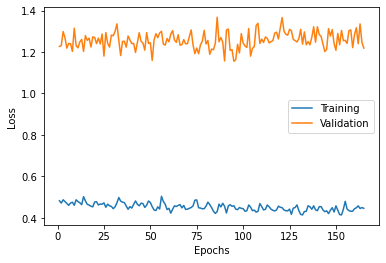
\includegraphics[width=\textwidth]{Latex template for Project Report-20220108/immagini/L2DropEarlyLoss.png}
         \caption{L2-Dr-ES Loss}
         \label{fig:L2DropESLoss}
     \end{subfigure}
     \hfill
     \begin{subfigure}[b]{0.32\textwidth}
         \centering
         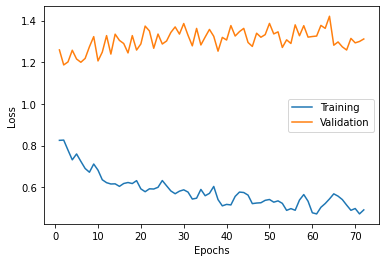
\includegraphics[width=\textwidth]{Latex template for Project Report-20220108/immagini/L2EarlyCWLoss.png}
         \caption{L2-ES-CW Loss}
         \label{fig:L2ESCWLoss}
     \end{subfigure}
     
      \begin{subfigure}[b]{0.32\textwidth}
         \centering
         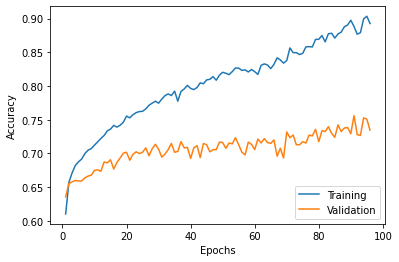
\includegraphics[width=\textwidth]{Latex template for Project Report-20220108/immagini/L2EarlyAccuracy.png}
         \caption{L2-ES Accuracy}
         \label{fig:L2ESAcc}
     \end{subfigure}
     \hfill
     \begin{subfigure}[b]{0.32\textwidth}
         \centering
         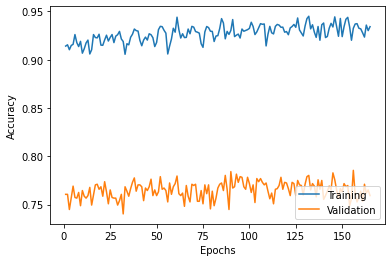
\includegraphics[width=\textwidth]{Latex template for Project Report-20220108/immagini/L2DropEarlyAccuracy.png}
         \caption{L2-Dr-ES Accuracy}
         \label{fig:L2DropESAcc}
     \end{subfigure}
     \hfill
     \begin{subfigure}[b]{0.32\textwidth}
         \centering
         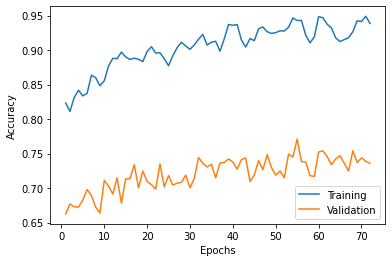
\includegraphics[width=\textwidth]{Latex template for Project Report-20220108/immagini/L2EarlyCWAccuracy.png}
         \caption{L2-ES-CW Acc}
         \label{fig:L2ESCWAcc}
     \end{subfigure}
     
     \begin{subfigure}[b]{0.32\textwidth}
         \centering
         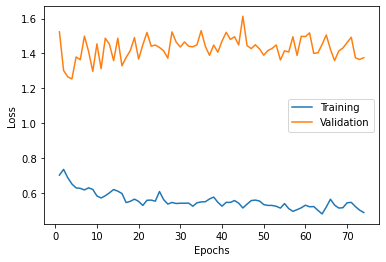
\includegraphics[width=\textwidth]{Latex template for Project Report-20220108/immagini/L2DropEarlyCWLoss.png}
         \caption{L2-Dr-ES-CW Loss}
         \label{fig:L2DropESCWLoss}
     \end{subfigure}
     \hspace{2em}
     \begin{subfigure}[b]{0.32\textwidth}
         \centering
         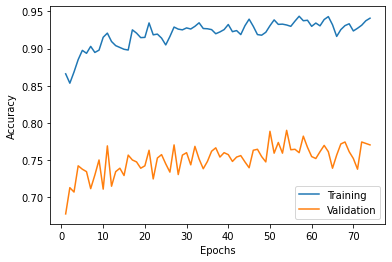
\includegraphics[width=\textwidth]{Latex template for Project Report-20220108/immagini/L2DropEarlyCWAccuracy.png}
         \caption{L2-Dr-ES-CW Acc}
         \label{fig:L2DropESCWAcc}
     \end{subfigure}
     
     \caption{Loss e accuracy dei modelli con combinazioni di regolarizzazione}
     \label{fig:secondiModelli}
\end{figure} 

Si può notare come tutti i modelli riportino risultati molto simili: ottimi valori di \textit{loss} e \textit{accuracy} sul train set, \textit{validation loss} intorno a 1.2-1.3 e \textit{validation accuracy} tra 0.75 e 0.80.

\begin{table}[h!]
\centering
\resizebox{.8\textwidth}{!}{%
        \begin{tabular}{| c | c | c | c | c |}
            \hline 
            Modello & Train Loss & Train Accuracy & Validation Loss & Validation Accuracy\\ \hline
            FAMD  & 0.006 & 0.999 & 2.594 & 0.749 \\ \hline
            OHE & 0.002 & 0.999 & 1.839 & 0.822 \\ \hline
            L1 & 0.391 & 0.961 & 1.377 & 0.793 \\ \hline
            L2 & 0.354 & 0.971 & 1.171 & 0.782 \\ \hline
            L2-Dropout & 0.498 & 0.910 & 1.208 & 0.764 \\ \hline
            L2-ES & 0.516 & 0.897 & 1.052 & 0.756 \\ \hline
            L2-Dropout-ES & 0.387 & 0.957 & 1.241 & 0.785 \\ \hline
            L2-ES-CW & 0.449 & 0.967 & 1.290 & 0.771 \\ \hline
            L2-Dropout-ES-CW & 0.405 & 0.971 & 1.363 & 0.790 \\ \hline
        \end{tabular}
        }
    \caption{Risultati all'ultima epoca su Train e Validation set}
    \label{tab:xxx}
\end{table}

Dall'osservazione dei grafici in Figura \ref{fig:primiModelli} e Figura \ref{fig:secondiModelli}, non avendo riscontrato alcun modello di spicco tra gli altri, ne sono stati selezionati tre per proseguire l'analisi dei loro risultati: \textit{L2}, \textit{L2 ES} (che riporta il più basso valore di \textit{accuracy loss} tra tutti i modelli) e \textit{L2 ES CW}.
Per questi, verranno infatti valutate alcune misure di performance su validation e test set, visibili in Tabella \ref{table:l2m}. 
È possibile notare come i valori ottenuti, per questi tre modelli, con il test set siano leggermente peggiori rispetto a quelli ottenuti con il validation set, ma molto simili. 
In particolare si osservano difficoltà nella predizione della classe 2, \textit{test accuracy} intorno a 0.74 e \textit{test loss} tra 1.20 e 1.60.

% \begin{figure}[H]
%         \centering
%      \begin{subfigure}[b]{0.27\textwidth}
%          \centering
%          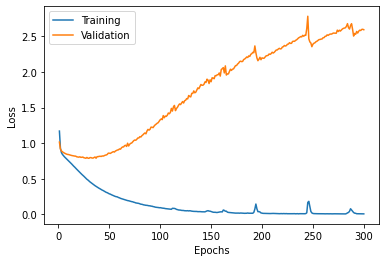
\includegraphics[width=\textwidth]{Latex template for Project Report-20220108/immagini/FAMDLoss.PNG}
%          %\captionsize{small}
%          \caption{FAMD Loss}
%          \label{fig:FAMDLoss}
%      \end{subfigure}
%      \hfill
%      \begin{subfigure}[b]{0.27\textwidth}
%          \centering
%          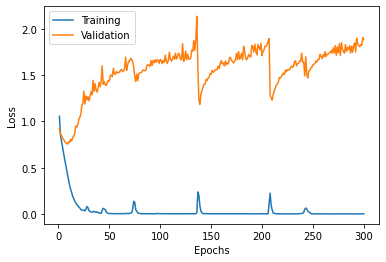
\includegraphics[width=\textwidth]{Latex template for Project Report-20220108/immagini/OHELoss.png}
%          \caption{OHE Loss}
%          \label{fig:OHELoss}
%      \end{subfigure}
%      \hfill
%      \begin{subfigure}[b]{0.27\textwidth}
%          \centering
%          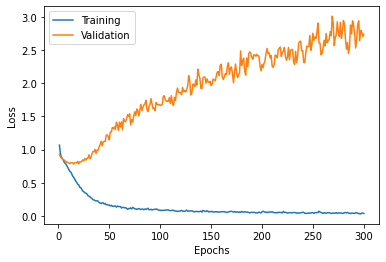
\includegraphics[width=\textwidth]{Latex template for Project Report-20220108/immagini/DropoutLoss.png}
%          \caption{Dropout Loss}
%          \label{fig:DropLoss}
%      \end{subfigure}
     
%      \begin{subfigure}[b]{0.27\textwidth}
%          \centering
%          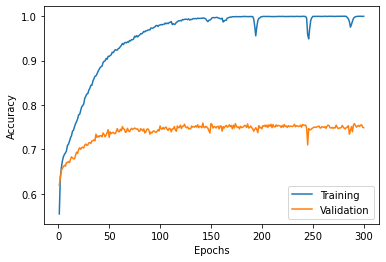
\includegraphics[width=\textwidth]{Latex template for Project Report-20220108/immagini/FAMDAccuracy.png}
%          \caption{FAMD Accuracy}
%          \label{fig:FAMDAcc}
%      \end{subfigure}
%      \hfill
%      \begin{subfigure}[b]{0.27\textwidth}
%          \centering
%          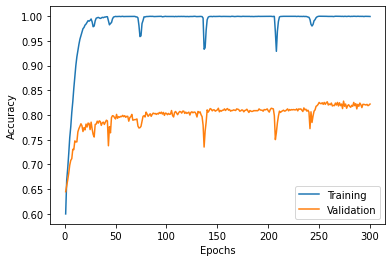
\includegraphics[width=\textwidth]{Latex template for Project Report-20220108/immagini/OHEAccuracy.png}
%          \caption{OHE Accuracy}
%          \label{fig:OHEAcc}
%      \end{subfigure}
%      \hfill
%      \begin{subfigure}[b]{0.27\textwidth}
%          \centering
%          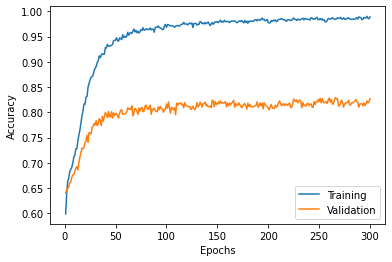
\includegraphics[width=\textwidth]{Latex template for Project Report-20220108/immagini/DropoutAccuracy.png}
%          \caption{Dropout Accuracy}
%          \label{fig:DropAcc}
%      \end{subfigure}

% \end{figure}




%Al fine di rendere ancora più chiaro il risultato ottenuto all'ultima epoca da ogni modello, sono stati riportati nella Tabella \ref{tab:xxx} i valori di \textit{loss} e \textit{accuracy} per train e validation set.


%%%%%%%%%%tabella multi row
% richiesti: 
% \usepackage{adjustbox}
% \usepackage{multirow}
% \begin{table}[h!]
% \centering
% \resizebox{.45\textwidth}{!}{%
%         \begin{tabular}{| c | c | c | c |}
%             \hline 
%             \multicolumn{1}{|c|}{Modello} & \multicolumn{1}{c|}{Set} & \multicolumn{1}{c|}{Loss} & \multicolumn{1}{c|}{Accuracy}\\ \hline
%             \multirow{2}{*}{FAMD}  &
%             \multicolumn{1}{l|}{Train} & \multicolumn{1}{l|}{0.006} & \multicolumn{1}{c|}{0.999} \\ \cline{2-4}
%                                       & \multicolumn{1}{l|}{Validation} & \multicolumn{1}{l|}{2.594} & \multicolumn{1}{c|}{0.749} \\ \hline
%             \multirow{2}{*}{OHE} & 
%             \multicolumn{1}{l|}{Train} & \multicolumn{1}{l|}{0.002} & \multicolumn{1}{c|}{0.999} \\ \cline{2-4}
%                                       & \multicolumn{1}{l|}{Validation} & \multicolumn{1}{l|}{1.839} & \multicolumn{1}{c|}{0.822} \\ \hline
%             \multirow{2}{*}{L1} &
%             \multicolumn{1}{l|}{Train} & \multicolumn{1}{l|}{0.391} & \multicolumn{1}{c|}{0.961} \\ \cline{2-4}
%                                       & \multicolumn{1}{l|}{Validation} & \multicolumn{1}{l|}{1.377} & \multicolumn{1}{c|}{0.793} \\ \hline
%             \multirow{2}{*}{L2} &
%             \multicolumn{1}{l|}{Train} & \multicolumn{1}{l|}{0.354} & \multicolumn{1}{c|}{0.971} \\ \cline{2-4}
%                                       & \multicolumn{1}{l|}{Validation} & \multicolumn{1}{l|}{1.171} & \multicolumn{1}{c|}{0.782} \\ \hline
%             \multirow{2}{*}{L2-Dropout} &
%             \multicolumn{1}{l|}{Train} & \multicolumn{1}{l|}{0.498} & \multicolumn{1}{c|}{0.910} \\ \cline{2-4}
%                                       & \multicolumn{1}{l|}{Validation} & \multicolumn{1}{l|}{1.208} & \multicolumn{1}{c|}{0.764} \\ \hline
%             \multirow{2}{*}{L2-ES} &
%             \multicolumn{1}{l|}{Train} & \multicolumn{1}{l|}{0.516} & \multicolumn{1}{c|}{0.897} \\ \cline{2-4}
%                                       & \multicolumn{1}{l|}{Validation} & \multicolumn{1}{l|}{1.052} & \multicolumn{1}{c|}{0.756} \\ \hline
%             \multirow{2}{*}{L2-Dropout-ES} &
%             \multicolumn{1}{l|}{Train} & \multicolumn{1}{l|}{0.387} & \multicolumn{1}{c|}{0.957} \\ \cline{2-4}
%                                       & \multicolumn{1}{l|}{Validation} & \multicolumn{1}{l|}{1.241} & \multicolumn{1}{c|}{0.785} \\ \hline
%             \multirow{2}{*}{L2-ES-CW} &
%             \multicolumn{1}{l|}{Train} & \multicolumn{1}{l|}{0.449} & \multicolumn{1}{c|}{0.967} \\ \cline{2-4}
%                                       & \multicolumn{1}{l|}{Validation} & \multicolumn{1}{l|}{1.290} & \multicolumn{1}{c|}{0.771} \\ \hline
%             \multirow{2}{*}{L2-Dropout-ES-CW} &
%             \multicolumn{1}{l|}{Train} & \multicolumn{1}{l|}{0.405} & \multicolumn{1}{c|}{0.971} \\ \cline{2-4}
%                                       & \multicolumn{1}{l|}{Validation} & \multicolumn{1}{l|}{1.363} & \multicolumn{1}{c|}{0.790} \\ \hline
%         \end{tabular}
%         }
%     \caption{Risultati all'ultima epoca su Train e Validation set}
%     \label{tab:xxx}
% \end{table}





%Si può notare come tutti i modelli riportino risultati molto simili: ottimi valori di \textit{loss} e \textit{accuracy} sul train set, \textit{validation loss} intorno a 1.2-1.3 e \textit{validation accuracy} tra 0.75 e 0.80.

%Dall'osservazione dei grafici in Figura \ref{fig:primiModelli} e Figura \ref{fig:secondiModelli}, non avendo riscontrato alcun modello di spicco tra gli altri, ne sono stati selezionati tre per proseguire l'analisi dei loro risultati: \textit{L2}, \textit{L2 EarlyStopping} (che riporta il più basso valore di \textit{accuracy loss} tra tutti i modelli) e \textit{L2 EarlyStopping ClassWeight}.
%Per questi, verranno infatti valutate alcune misure di performance su validation e test set, visibili in Tabella \ref{table:l2m}. 

% \begin{figure}[H]
%      \centering
%      \begin{subfigure}[b]{0.3\textwidth}
%          \centering
%          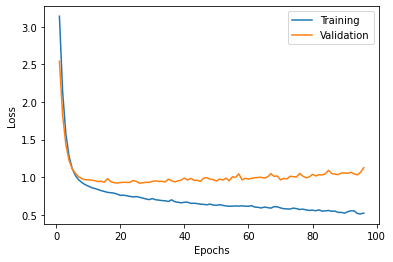
\includegraphics[width=\textwidth]{Latex template for Project Report-20220108/immagini/L2EarlyLoss.png}
%          \caption{L2-ES Loss}
%          \label{fig:L2ESLoss}
%      \end{subfigure}
%      \hspace{2em}
%      \begin{subfigure}[b]{0.3\textwidth}
%          \centering
%          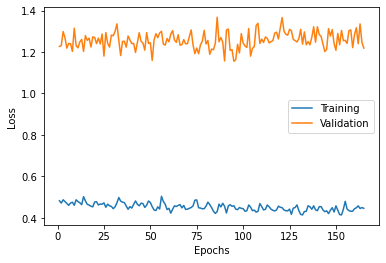
\includegraphics[width=\textwidth]{Latex template for Project Report-20220108/immagini/L2DropEarlyLoss.png}
%          \caption{L2-Dr-ES Loss}
%          \label{fig:L2DropESLoss}
%      \end{subfigure}
     
%      \begin{subfigure}[b]{0.3\textwidth}
%          \centering
%          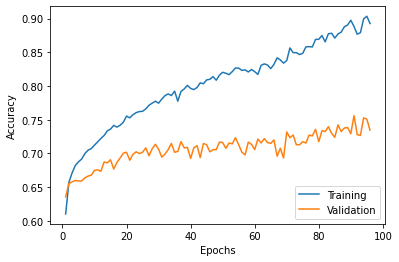
\includegraphics[width=\textwidth]{Latex template for Project Report-20220108/immagini/L2EarlyAccuracy.png}
%          \caption{L2-ES Accuracy}
%          \label{fig:L2ESAcc}
%      \end{subfigure}
%      \hspace{2em}
%      \begin{subfigure}[b]{0.3\textwidth}
%          \centering
%          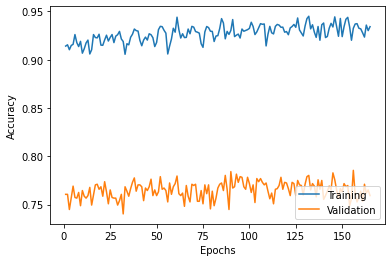
\includegraphics[width=\textwidth]{Latex template for Project Report-20220108/immagini/L2DropEarlyAccuracy.png}
%          \caption{L2-Dr-ES Accuracy}
%          \label{fig:L2DropESAcc}
%      \end{subfigure}
     
%      \begin{subfigure}[b]{0.3\textwidth}
%          \centering
%          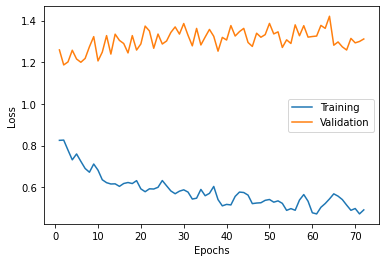
\includegraphics[width=\textwidth]{Latex template for Project Report-20220108/immagini/L2EarlyCWLoss.png}
%          \caption{L2-ES-CW Loss}
%          \label{fig:L2ESCWLoss}
%      \end{subfigure}
%      \hspace{2em}
%      \begin{subfigure}[b]{0.3\textwidth}
%          \centering
%          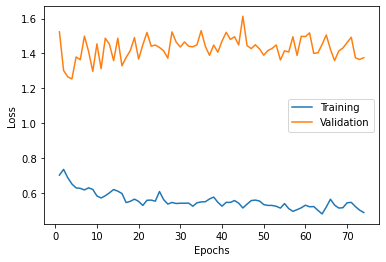
\includegraphics[width=\textwidth]{Latex template for Project Report-20220108/immagini/L2DropEarlyCWLoss.png}
%          \caption{L2-Dr-ES-CW Loss}
%          \label{fig:L2DropESCWLoss}
%      \end{subfigure}
     
%      \begin{subfigure}[b]{0.3\textwidth}
%          \centering
%          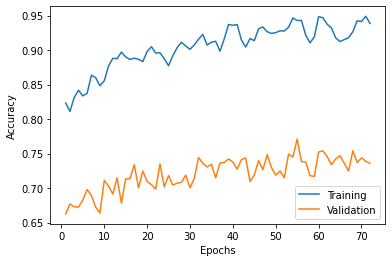
\includegraphics[width=\textwidth]{Latex template for Project Report-20220108/immagini/L2EarlyCWAccuracy.png}
%          \caption{L2-ES-CW Acc}
%          \label{fig:L2ESCWAcc}
%      \end{subfigure}
%      \hspace{2em}
%      \begin{subfigure}[b]{0.3\textwidth}
%          \centering
%          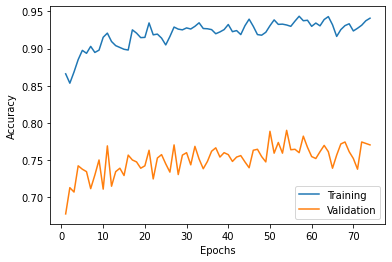
\includegraphics[width=\textwidth]{Latex template for Project Report-20220108/immagini/L2DropEarlyCWAccuracy.png}
%          \caption{L2-Dr-ES-CW Acc}
%          \label{fig:L2DropESCWAcc}
%      \end{subfigure}
     
%      \caption{Loss e accuracy dei modelli ottenuti combinando diverse tecniche di regolarizzazione}
%         %\label{fig:three graphs}
% \end{figure}






% \begin{table}[H]
% \centering
%         \begin{tabular}{| c | c | c | c |}
%             \hline 
%             \multicolumn{1}{|c|}{Modello} & \multicolumn{1}{c|}{Set} & \multicolumn{1}{c|}{Loss} & \multicolumn{1}{c|}{Accuracy}\\ \hline
%             \multirow{2}{*}{FAMD}  &
%             \multicolumn{1}{l|}{Train} & \multicolumn{1}{l|}{0.006} & \multicolumn{1}{l|}{0.999} \\ \cline{2-4}
%                                       & \multicolumn{1}{l|}{Validation} & \multicolumn{1}{l|}{2.594} & \multicolumn{1}{l|}{0.749} \\ \hline
%             \multirow{2}{*}{OHE} & 
%             \multicolumn{1}{l|}{Train} & \multicolumn{1}{l|}{0.002} & \multicolumn{1}{l|}{0.999} \\ \cline{2-4}
%                                       & \multicolumn{1}{l|}{Validation} & \multicolumn{1}{l|}{1.839} & \multicolumn{1}{l|}{0.822} \\ \hline
%             \multirow{2}{*}{L1} &
%             \multicolumn{1}{l|}{Train} & \multicolumn{1}{l|}{0.391} & \multicolumn{1}{l|}{0.961} \\ \cline{2-4}
%                                       & \multicolumn{1}{l|}{Validation} & \multicolumn{1}{l|}{1.377} & \multicolumn{1}{l|}{0.793} \\ \hline
%             \multirow{2}{*}{L2} &
%             \multicolumn{1}{l|}{Train} & \multicolumn{1}{l|}{0.354} & \multicolumn{1}{l|}{0.971} \\ \cline{2-4}
%                                       & \multicolumn{1}{l|}{Validation} & \multicolumn{1}{l|}{1.171} & \multicolumn{1}{l|}{0.782} \\ \hline
%             \multirow{2}{*}{L2-Dropout} &
%             \multicolumn{1}{l|}{Train} & \multicolumn{1}{l|}{0.498} & \multicolumn{1}{l|}{0.910} \\ \cline{2-4}
%                                       & \multicolumn{1}{l|}{Validation} & \multicolumn{1}{l|}{1.208} & \multicolumn{1}{l|}{0.764} \\ \hline
%             \multirow{2}{*}{L2-Early Stopping} &
%             \multicolumn{1}{l|}{Train} & \multicolumn{1}{l|}{0.516} & \multicolumn{1}{l|}{0.897} \\ \cline{2-4}
%                                       & \multicolumn{1}{l|}{Validation} & \multicolumn{1}{l|}{1.052} & \multicolumn{1}{l|}{0.756} \\ \hline
%             \multirow{2}{*}{L2-Dropout-Early Stopping} &
%             \multicolumn{1}{l|}{Train} & \multicolumn{1}{l|}{0.387} & \multicolumn{1}{l|}{0.957} \\ \cline{2-4}
%                                       & \multicolumn{1}{l|}{Validation} & \multicolumn{1}{l|}{1.241} & \multicolumn{1}{l|}{0.785} \\ \hline
%             \multirow{2}{*}{L2-Early Stopping-Class Weight} &
%             \multicolumn{1}{l|}{Train} & \multicolumn{1}{l|}{0.449} & \multicolumn{1}{l|}{0.967} \\ \cline{2-4}
%                                       & \multicolumn{1}{l|}{Validation} & \multicolumn{1}{l|}{1.290} & \multicolumn{1}{l|}{0.771} \\ \hline
%             \multirow{2}{*}{L2-Dropout-Early Stopping-Class Weight} &
%             \multicolumn{1}{l|}{Train} & \multicolumn{1}{l|}{0.405} & \multicolumn{1}{l|}{0.971} \\ \cline{2-4}
%                                       & \multicolumn{1}{l|}{Validation} & \multicolumn{1}{l|}{1.363} & \multicolumn{1}{l|}{0.790} \\ \hline
%         \end{tabular}
%     \caption{Risultati su Train e Validation set}
%     \label{tab:xxx}
% \end{table}



\begin{table}[h!]
    \parbox{.45\textwidth}{
        \centering
        \begin{adjustbox}{max width=.45\textwidth}
        \begin{tabular}{|c|c|c|c|c|}
        \hline
            \multicolumn{5}{| c |}{L2 Validation Set} \\ \hline
            &  precision &   recall & f1-score  &  support \\ \hline
            0   &     0.56   &    0.74  &    0.64    &    93 \\ \hline
            1   &     0.58   &    0.60  &    0.59    &    253\\ \hline
            2   &     0.56   &    0.36  &    0.44    &    306\\ \hline
            3   &     0.84   &    0.91  &    0.87    &    877\\ \hline
            accuracy   &       &        &    0.74   &   1529 \\ \hline
            loss   &     &     & 1.31   &   1529\\ \hline
            macro avg   &    0.63     & 0.65   &   0.63   &   1529 \\ \hline
            weighted avg   &    0.72    &  0.74     & 0.72   &   1529\\ \hline
        \end{tabular}
        \end{adjustbox}
    }
    \hfill
    \parbox{.45\textwidth}{
    \begin{adjustbox}{max width=.45\textwidth}
    \centering
        \begin{tabular}{|c|c|c|c|c|}
                \hline
                \multicolumn{5}{| c |}{L2 Test Set} \\ \hline
                 & precision &   recall & f1-score  &  support \\ \hline
                    0    &    0.64    &   0.75     &  0.69    &    140 \\ \hline
                   1    &   0.60    &  0.58    &  0.59    &   318\\ \hline
                   2    &   0.56    &  0.38   &   0.45    &   376\\ \hline
                   3    &   0.82    &  0.90   &   0.85   &  1078\\ \hline
            accuracy    &       &        &    0.73    &  1912\\ \hline
            loss   &     &     & 1.59   &   1912\\ \hline
           macro avg    &   0.65    &  0.65  &    0.65    &  1912\\ \hline
        weighted avg    &   0.72   &   0.73  &    0.72   &   1912\\ \hline
            \end{tabular}
            \end{adjustbox}
    }

    \vspace{.2cm}
    \parbox{.45\textwidth}{
        \centering
        \begin{adjustbox}{max width=.45\textwidth}
        \begin{tabular}{|c|c|c|c|c|}
        \hline
            \multicolumn{5}{| c |}{L2-Early Stopping Validation Set} \\ \hline
            &  precision &   recall & f1-score  &  support \\ \hline
            0   &    0.32    &  0.68    &  0.43    &    57\\ \hline
            1   &    0.57    &  0.57    &  0.57    &   263\\ \hline
            2   &    0.45   &   0.41    &  0.43     &  212\\ \hline
            3    &   0.93   &   0.88    &  0.91    &  997\\ \hline
            accuracy    &    &        &           0.76    &  1529\\ \hline
            loss   &     &     & 1.05   &   1529\\ \hline
            macro avg    &   0.57    &  0.64   &   0.58    &  1529\\ \hline
            weighted avg    &   0.78  &    0.76   &   0.76   &   1529 \\ \hline
        \end{tabular}
        \end{adjustbox}
    }
    \hfill
    \parbox{.45\textwidth}{
    \begin{adjustbox}{max width=.45\textwidth}
    \centering
        \begin{tabular}{|c|c|c|c|c|}
                \hline
                \multicolumn{5}{| c |}{L2-Early Stopping Test Set} \\ \hline
                 & precision &   recall & f1-score  &  support \\ \hline
                0  &     0.34   &   0.63    &  0.44   &     87\\ \hline
                1    &   0.53   &   0.49    &  0.51 &      335\\ \hline
                2    &   0.46   &   0.41    &  0.43 &      285\\ \hline
                3    &   0.89   &   0.88    &  0.89 &     1205\\ \hline
                accuracy   &    &   &  0.73   &   1912\\ \hline
                loss   &     &     & 1.20   &   1912\\ \hline
                macro avg   &    0.55   &   0.60  &    0.57   &   1912\\ \hline
                weighted avg   &    0.74    &  0.73    &  0.73   &   1912\\ \hline
            \end{tabular}
            \end{adjustbox}
    }
    
    \vspace{.2cm}
    \parbox{.45\textwidth}{
        \centering
        \begin{adjustbox}{max width=.45\textwidth}
        \begin{tabular}{|c|c|c|c|c|}
        \hline
            \multicolumn{5}{| c |}{L2-Early Stopping-Class Weight Validation Set} \\ \hline
            &  precision &   recall & f1-score  &  support \\ \hline
            0   &    0.50  &    0.82  &    0.62   &     76\\ \hline
            1   &    0.66  &    0.63  &    0.64   &    276\\ \hline
            2   &    0.62  &    0.43  &    0.51   &    284\\ \hline
            3   &    0.87  &    0.92  &    0.89   &    893\\ \hline
            accuracy   &    &         &    0.77   &   1529\\ \hline
            loss   &     &     & 1.29   &   1529\\ \hline
            macro avg  & 0.66  &  0.70 & 0.67   &   1529\\ \hline
            weighted avg   &     0.77    &   0.77    &   0.76    &   1529\\ \hline
        \end{tabular}
        \end{adjustbox}
    }
    \hfill
    \parbox{.45\textwidth}{
    \begin{adjustbox}{max width=.45\textwidth}
    \centering
        \begin{tabular}{|c|c|c|c|c|}
                \hline
                \multicolumn{5}{| c |}{L2-Early Stopping-Class Weight Test Set} \\ \hline
                 & precision &   recall & f1-score  &  support \\ \hline
                0   &    0.55  &    0.73  &    0.63   &    124\\ \hline
                1   &    0.59  &    0.56  &    0.58   &    329\\ \hline
                2   &    0.60  &    0.42  &    0.50   &    359\\ \hline
                3   &    0.84  &    0.91  &    0.87   &   1100\\ \hline
                accuracy   &    &         & 0.75   &   1912\\ \hline
                loss   &     &     & 1.56   &   1912\\ \hline
                macro avg    &   0.65   &   0.66   &   0.65   &   1912\\ \hline
                weighted avg    &   0.74    &  0.75    &  0.74   &   1912\\ \hline
            \end{tabular}
            \end{adjustbox}
    }
        \caption{Risultati Validation e Test set}
        \label{table:l2m}
\end{table}

%È possibile notare come i valori ottenuti, per questi tre modelli, con il test set siano leggermente peggiori rispetto a quelli ottenuti con il validation set, ma molto simili. 
%In particolare si osservano difficoltà nella predizione della classe 2, \textit{test accuracy} intorno a 0.74 e \textit{test loss} tra 1.20 e 1.60.